\section{Alternative Metrics}

Since BLEU did not reflect well the semantic similarity of migrated
code and reference code, there is a need for an alternative metric
that can fit better with the task. The nature of the task is to
compare source code in term of program semantics with respect to a
programming language.
%
%To compare the two language bases, they must be represented in some
%ways. 
While a language is normally composed by three important parts:
vocabulary, grammar, and meaning; programming language can be composed
by the three corresponding parts: lexeme, syntax, and
semantics. 
%
Therefore, we consider three representations that reflect each of the
three above parts. Specifically, we use tokens, Abstract Syntax Trees
(ASTs), and Program Dependence Graphs (PDGs) in this study to estimate
the semantic accuracy of the migrated code from SMT-based migration
tools.
%choose one representation for each of the above part to
%compare, in order to heuristically estimate the semantic
%similarity. 
%Specifically, token, AST and PDG are representations of lexemes,
%syntax, and semantics respectively. 
%
Let us explain the metrics to compare the three above representations.
%
%The metrics to compare those representations are SED, TREED and GVED
%which are defined below. Those metrics are then evaluated to show how
%well they reflect Semantic score.
We then present our experiments to evaluate the correlation between
each of the metrics and the semantic scores.


\subsection{Definitions}

\subsubsection{\textbf{String Edit Distance (SED)}}
String Edit Distance (SED) is the metric to compare source code when
it is represented as sequence of tokens. SED measures efforts that a
user must edit in term of the tokens that need to be deleted/added to
transform the resulting code into the correct one. In our study, we
used Levenshtein algorithm to calculate that distance. The metric is
normalized as: $SED = 1 - \frac{EditDistance\left(s_R,
  s_T\right)}{length\left(s_R\right)}$ where $s_R$ is the sequence of
tokens representing the reference code; $s_T$ is the sequence of
tokens represent the translated code; $EditDistance\left(s_R,
s_T\right)$ is the editing distance between the pair; and the
denominator is the total length of the reference code. For example,
$EditDistance\left(s_R, s_T\right)$ between translated code and
reference code in Figure~\ref{fig:issueexample2} is 4 (two deletions,
two additions). Then, it is normalized as 0.952. Note that the closer
the score to 1, the more similar the pair in term of lexical~tokens.

\subsubsection{\textbf{Tree Edit Distance (TREED)}}  
The sematical quality of translated code depends on its syntax. Until now, abstract syntax trees(AST) are structures widely used in  representing the syntax of programming code. Therefore, computing the difference of two ASTs is considered as the evaluating method of syntax difference.
In this study, we apply this in measuring the difference between the syntax of referenced method and translated method. Given a pair of method in C\# which are need to be compared their syntax, Roslyn[cite here] is used to parse them into ASTs. Then we compute the tree edit distance between two trees using the algorithm Treed described in the paper \cite{algorithm}.
To be more detailed, the tree edit distance is calculated by number of operations (add/delete/replace/move) to make them identical. 

It is computed as:  $TREED = 1 -  \frac{TreeEditDistance\left(AST_R, AST_T\right)}{CountNodes \left(AST_R+AST_T\right)}$ where $TreeEditDistance\left(AST_R, AST_T\right)$ is the editing distance between two trees of referenced method $AST_R$ and the translated method $AST_T$; and the denominator is the total nodes in the tree of both two methods. The value of TREED is from 0 to 1. For any two trees, there will always exist at least one editing (such as the one that deletes all nodes of the first tree and inserts all the nodes of the second). Therefore, there will always exist at least one TREED value and the higher value is, the more similar those trees are.

\begin{figure}[h]
	\caption{Tree Editing Example: In the label of each node, its type is in capital font and its val (if exists) is in normal font}
	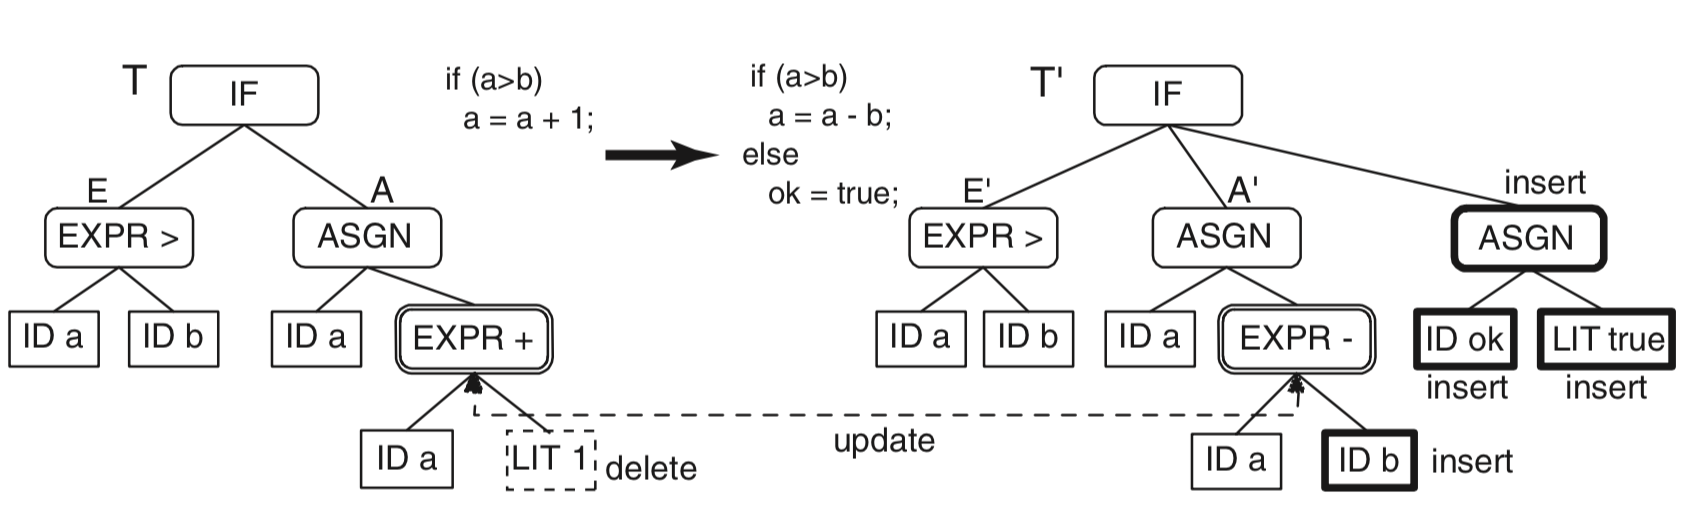
\includegraphics[scale=0.3]{img/treed.png}
	\centering
	\label{fig:treed}
\end{figure}

In the example in Figure 1, an \textit{if} statement was edited by modifying the \textit{if} branch and adding an \textit{else} branch. The two trees represent the two versions of a method. An editing consists of one \textit{Delete} (dotted line box), one \textit{Update} (double-line box), and four \textit{Insert} operations (bold boxes). Other nodes (single- line boxes) are either unchanged or moved. Based on the formula TREED, the result of TREED in this case  $TREED = 1 - \frac{1 + 1 + 4}{16}=0.625$





\subsubsection{\textbf{Graph Vector Edit Distance (GVED)}} 

Structure-oriented approaches in code semantic comparision have become
popular. Among those approaches, Exas is an accurate and efficient
structural characteristic feature extraction approach that better
approximates and captures the structure within the fragments of
artifacts~\cite{fase09}.  In our study, we use Exas as a mean of
computing the difference between code structures. Given a pair of
method in C\# which are need to be compared their structure, program
dependence graphs (PDGs) are built with some additional nodes from
GROUM~\cite{fse09}. Exas vectors will be computed on those graphs. In
Exas, the characteristic features are extracted from the patterns of
elements of the graphs. The code fragments are characterized by their
counting vectors of those features. The difference between two vectors
reflects the difference of two graphs.

%Therefore, distance of these counting vectors is considered the way to measure the sematic between code fragments.

Figure~\ref{fig:PDGs} shows the PDGs of the code fragments 1 and
2. These graphs are analysed by Exas, which focuses on two kinds of
patterns of structural information of the graph, called $(p,q)$-node
and $n$-path as can be seen in Table~\ref{tab:feature1} and
Table~\ref{tab:feature2}.

An efficient way to express the property ``having the same or similar
features'' is to use vectors. The characteristic vector of a
fragment is the occurrence-count vector of its features. That is, each
position in the vector is indexed for a feature and the value at that
position is the number of occurrences of that feature in the
fragment. Table~\ref{tab:featureIndex} shows the indexes of the
features, which are global across all vectors. Based on the occurrence
counts, the vectors for code fragment 1 and 2 are
$V_1$(1,1,1,1,1,0,1,0...),$V_2$(1,1,0,1,1,1,1,1...), respectively. Two
fragments having the same feature sets and occurrence counts will have
the same vectors and vice versa. The vector similarity can be measured
by a chosen vector distance such as 1-norm distance.

We introduce the formula for normalizing the result of vector edit
distance which is used in our experiments. The normalized
value is described as
\[GVED \left( V_1, V_2 \right) = 1 - \sum_{i=1}^{n} \frac{ \mid XV1_i - XV2_i \mid}{XV1_i + XV2_i}\], 
where $n$ denotes the number of vector scalar, $V_1$ denotes the
counting vector of the first graph, $V_2$ denotes the counting vector
of the second graph, $XV1_i$ denotes $V_1$\rq the value of the ($i-th$)
scalar, $XV2_i$ denotes $V2$\rq the value of the ($i-th$) scalar.

In this example in Figure~\ref{code1code2}, the value of GVED is $GVED\left(V_1, V_2\right) = 1 - \frac{8 }{20} = 0.6 $,

\begin{figure}
\begin{lstlisting}[language=JAVA]
	Code 1:
	void foo(int i) {
		int j;
		if (i < 2) {
			j = 1;
		} else {
			j = 2;
		}
	}

	Code 2:
	void foo(int i) {
		int j;
		if (i < 2) 
			j = i;	 
		j = 2;
	}
\end{lstlisting}
\caption{Example of two code fragments}
\label{code1code2}
\end{figure}

\begin{figure}[h]
	\caption{An example: two PDGs represent code1 and code2}
	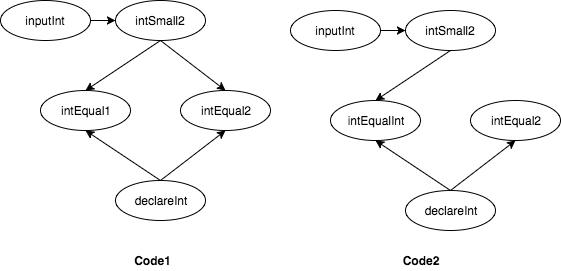
\includegraphics[scale=0.4]{img/Diagram_PDG.png}
	\centering
	\label{fig:PDGs}
\end{figure}

% Table generated by Excel2LaTeX from sheet 'Sheet1'
\begin{table}[htbp]
  \centering
  \caption{Feature table of code1 extracted in Exas}
  \scalebox{0.65}{
    \begin{tabular}{|l|l|l|l|l|r|}
    \toprule
    \textbf{Pattern} & \multicolumn{5}{c|}{\textbf{Feature of Code1}} \\
    \midrule
    \textit{\textbf{1-path}} & inputInt & intSmall2 & intEqual1 & intEqual2 & \multicolumn{1}{l|}{declareInt} \\
    \midrule
    \textit{\textbf{2-path}} & \multicolumn{1}{p{6.415em}|}{inputInt-intSmall2} & \multicolumn{1}{p{5.915em}|}{intSmall2-intEqual1} & \multicolumn{1}{p{6em}|}{intSmall2-intEqual2} & \multicolumn{1}{p{5.75em}|}{declareInt-intEqual1} & \multicolumn{1}{p{5em}|}{declareInt-intEqual2} \\
    \midrule
    \textit{\textbf{3-path}} & \multicolumn{1}{p{6.415em}|}{intputInt-intSmall2-intEqual1} & \multicolumn{1}{p{5.915em}|}{intputInt-intSmall2-intEqual2} &       &       &  \\
    \midrule
    \textit{\textbf{(p,q)-node}} & inputInt-0-1 & intSmall2-1-2 & intEqual1-2-0 & intEqual2-1-2 &  \\
    \bottomrule
    \end{tabular}%
	}
  \label{tab:feature1}%
\end{table}%

% Table generated by Excel2LaTeX from sheet 'Sheet1'
\begin{table}[htbp]
  \centering
	\caption{Feature table of code2 extracted in Exas}
	\scalebox{0.65}{
	    \begin{tabular}{|l|l|l|l|l|r|}
    \toprule
    \textbf{Pattern} & \multicolumn{5}{c|}{\textbf{Feature of Code2}} \\
    \midrule
    \textit{\textbf{1-path}} & inputInt & intSmall2 & intEqualInt & intEqual2 & \multicolumn{1}{l|}{declareInt} \\
    \midrule
    \textit{\textbf{2-path}} & \multicolumn{1}{p{6.415em}|}{inputInt-intSmall2} & \multicolumn{1}{p{5.915em}|}{intSmall2-intEqualInt} & \multicolumn{1}{p{6em}|}{declareInt-intEqual1} & \multicolumn{1}{p{5.75em}|}{declareInt-intEqual2} &  \\
    \midrule
    \textit{\textbf{3-path}} & \multicolumn{1}{p{6.415em}|}{intputInt-intSmall2-intEqualInt} &       &       &       &  \\
    \midrule
    \textit{\textbf{(p,q)-node}} & inputInt-0-1 & intSmall2-1-1 & intEqualInt-2-0 & intEqual2-1-0 &  \\
    \bottomrule
    \end{tabular}%
	}
  \label{tab:feature2}%
\end{table}%

% Table generated by Excel2LaTeX from sheet 'Sheet1'
\begin{table}[htbp]
	\centering
	\caption{Feature Indexing}
	\scalebox{0.75}{
	\begin{tabular}{|cccc|}
		\toprule
		\multicolumn{1}{|l|}{\textbf{Feature}} & \multicolumn{1}{l|}{\textbf{Index}} & \multicolumn{1}{l|}{\textbf{Counted in Code1}} & \multicolumn{1}{l|}{\textbf{Counted in Code2}} \\
		\midrule
		\multicolumn{1}{|l|}{inputInt} & \multicolumn{1}{r|}{1} & \multicolumn{1}{r|}{1} & \multicolumn{1}{r|}{1} \\
		\midrule
		\multicolumn{1}{|l|}{intSmall2} & \multicolumn{1}{r|}{2} & \multicolumn{1}{r|}{1} & \multicolumn{1}{r|}{1} \\
		\midrule
		\multicolumn{1}{|l|}{intEqual1} & \multicolumn{1}{r|}{3} & \multicolumn{1}{r|}{1} & \multicolumn{1}{r|}{0} \\
		\midrule
		\multicolumn{1}{|l|}{intEqual2} & \multicolumn{1}{r|}{4} & \multicolumn{1}{r|}{1} & \multicolumn{1}{r|}{1} \\
		\midrule
		\multicolumn{1}{|l|}{declareInt} & \multicolumn{1}{r|}{5} & \multicolumn{1}{r|}{1} & \multicolumn{1}{r|}{1} \\
		\midrule
		\multicolumn{1}{|l|}{intEqualInt} & \multicolumn{1}{r|}{6} & \multicolumn{1}{r|}{0} & \multicolumn{1}{r|}{1} \\
		\midrule
		\multicolumn{1}{|p{5.75em}|}{inputInt-intSmall2} & \multicolumn{1}{r|}{7} & \multicolumn{1}{r|}{1} & \multicolumn{1}{r|}{1} \\
		\midrule
		\multicolumn{1}{|l|}{intEqual2-1-0} & \multicolumn{1}{r|}{8} & \multicolumn{1}{r|}{0} & \multicolumn{1}{r|}{1} \\
		\midrule
		\multicolumn{4}{|c|}{To be continued} \\
		\bottomrule
	\end{tabular}%
	}
	\label{tab:featureIndex}%
\end{table}%

 
\subsection{Experimental results on alternative metrics}

%To further study the relations between each of the three above metrics
%and the semantic scores, we conducted several experiments in the same
%manner as the previous study described in
%Section~\ref{sec:bleuresult}. We then present our proposed metric
%in Section~7 based on the results of the following experiments.

To evaluate the abilities of STS, TRS and GRS in reflecting the
semantic accuracy of translated code, we conducted three experiments
for these three metrics in the same manner as the study described in
Section~\ref{sec:bleuresult}.

The correlation coefficient results between each of the three metrics
with semantic score are described in
Table~\ref{table:correlation}. These results follow a similar trend:
for each model, the correlation coefficients increase 
according the abstraction levels of source code from text, syntax, to semantic
representations in three metrics. For example, for mppSMT, the correlation
coefficient between STS and semantic score is 0.549, whereas that
for TRS is much greater at 0.820. The highest value is the
correlation coefficient between GRS and semantic score at 0.910. A
reason for this phenomenon is that for a pair of source code, if they
are textually identical, they have the same AST representation, and
the exact-match in AST leads to the equivalence between the
corresponding PDGs. Meanwhile, the equivalence in a higher
abstraction level does not necessarily lead to the equivalence in a
lower abstraction. For example, Fig.~\ref{fig:mppSMT_example} shows
two methods with equivalent PDGs, but with textually~different. 

%Despite of the increase of the correlation coefficients, GRS and TRS
%are used to measure subsets of methods in our sample set 
%(table \ref{table:metrics}), and the sizes of GRS are greater than 
%TRS's ones, whereas STS is able to apply for all cases. For example, 
%the applicable sets of methods translated by lpSMT are quite limited, 
%75 and 123 (out of 375 methods) for GRS and TRS respectively. The reason
%for this phenomenon is that to construct the higher level representations,
%the translated results need to satisfy certain syntactic and semantic related
%constraints such as resolvable data and control dependencies.
%\begin{table}
%\centering
%\caption{Numbers of applicable methods of metrics}
%\begin{tabular}{|c|c|c|}
%\hline
%  & GRS & TRS\\
%\hline
%GNMT  & 128 & 155  \\
%\hline
%mppSMT  & 239 & 292 \\
%\hline
%lpSMT & 75 & 123 \\
%\hline
%\end{tabular}
%\label{table:metrics}
%\end{table}

Based on these empirical results, we conclude that the metric that
measures the results in the higher abstraction level, the better
metric for reflecting the semantics accuracy. However, the higher
representation like PDG cannot always be constructed because of
missing syntactic or semantic related information in the translated
results that is required to construct ASTs and PDGs. For example, the
sets of methods that are translated by lpSMT, and applicable for GRS
and TRS are quite limited, 75 and 123 (out of 375 methods),
respectively (the respective numbers for mppSMT are 239 and 292, and
those for GNMT are 128 and 155). Therefore, in
Section~\ref{sec:proposal}, we propose a metric to evaluate the
quality of translated code, that uses the measurement of the
similarity of translated code and expected results in multiple
representations.

%It is not worth to use SED instead of BLEU since it still has the same
%problems as BLEU while its advantage is insignificant.
%We then present our proposed metric in section~7 based on the results of the following experiments.

%To verify the 3 metrics SED, TREED, and GVED , we conducted an exploratory study that reveals their correlation with the ground truth Semantic score. Table \ref{table:correlation} summarizes our results for the two models mppSMT and lpSMT. We will explain each metric \rq s correlation in details as follows:

\begin{table}
\centering
\caption{Correlation between each metric with  semantic score on three models}
\begin{tabular}{|c|c|c|c|c|}
\hline
 & STS & TRS & GRS\\
\hline
mppSMT  & 0.549 & 0.820 & 0.910 \\
\hline
lpSMT  & 0.533 & 0.786 & 0.823 \\
\hline
GNMT & 0.692 & 0.734 & 0.927 \\
\hline
\end{tabular}
\label{table:correlation}
\end{table}


%\subsubsection{\textbf{SED vs Semantic}}
%
%SED is similar to BLEU in the way that both of them compare source
%code in term of lexical representation. Indeed, the two metrics have
%similar correlations with Semantic score
%(Table~\ref{table:correlation}). The correlation coefficient between SED and Semantic score is 0.549,
% 0.533, and 0.692 for three models mppSMT, lpSMT, and GNMT respectively.
%%equivalent 0.523 and 0.549 (mppSMT), and 0.67 and 0.675 (lpSMT). SED
%SED suffers the same drawbacks as BLEU: it does not take into
%consideration the structures of source code, and it compares source
%code only in term of lexical tokens.
%It is not worth to use SED instead of BLEU since it still has the same
%problems as BLEU while its advantage is insignificant.

%\begin{figure}
%\caption{SED vs Semantic (lpSMT)}
%\centering
%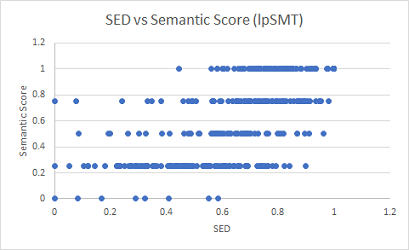
\includegraphics{img/sedvssem_lpSMT.png}
%\label{fig:SedSemlpSMT}
%\end{figure}
%
%\begin{figure}
%\caption{SED vs Semantic (mppSMT)}
%\centering
%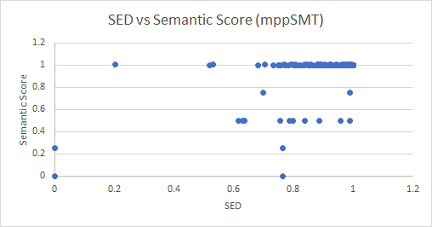
\includegraphics{img/sedvssem_mppSMT.png}
%\label{fig:SedSemMppSMT}
%\end{figure}

%\subsubsection{\textbf{TREED vs Semantic}}
%TREED compares source code at higher level of representation (Syntax Tree). Syntax of source code is the pre-requisite before mentioning about its semantics or functionality. Comparing methods in term of syntax is likely to reflect semantic accuracy better than comparing at lexical level. This argument is proved by our empirical results:

%Technically, a translated method cannot be said to perform any functionality if it cannot be compiled. However, in the Code Migration problem, a translated method which has wrong syntax can still be useful for developers.

%Figure \ref{fig:TREEDmppSMT} shows the scatter plots between 2
%metrics: TREED and Semantic score for the model mppSMT. In general, the result has similar
%trend as in the relation of BLEU and Semantic score: the data points
%are too scattered to show a strong correlation and there are
%several outliers. For a fixed value of Semantic score, TREED score can
%still vary in a large range. However, compared to BLEU, the variation
%is much smaller. For example, a pair of method that has Semantic score
%of 0.5 can possibly have TREED scores in range of 0.7 to 1 while such
%range is 0.5 to 1 for BLEU. TREED shows noticeable improvement over
%BLEU or SED on the correlation with Semantic score on the mppSMT model
%(0.549 to 0.820), on lpSMT model (0.533 to 0.786), and on the GNMT model (0.692 to 0.734).

%\emph{Observation 1:} For a fixed value of Semantic score, there can be many associated TREED values. Specifically, in the model lpSMT, with a Semantic Score of 1, the TREED scores can be varied greatly between 0-1, which was reflected on the top horizontal line of dots in figure \ref{fig:TREEDlpSMT}. Similarly, in the figure \ref{fig:TREEDmppSMT}, with a Semantic Score of 1, the TREED scores are in the range of 0.7 to 1.
%
%\emph{Observation 2:} For a fixed value of TREED, there can be many associated Semantic scores. For example, the figure \ref{fig:TREEDlpSMT} shows that for a high TREED score, for example 0.8, can have Semantic Score from 0.25 to 1. This can be observed by the vertical line of dots in the figure.



% Comparing figure \ref{fig:BleuSemMppSMT} and figure \ref{fig:TREEDmppSMT}, it can be realized that on the model mppSMT, those horizontal lines of dots in figure \ref{fig:BleuSemMppSMT} became shorter in figure \ref{fig:TREEDmppSMT}. It means the variation of TREED score for certain Semantic score is lower. Data points in the figure can also be approximately fitted with a regression line even though there still are some outliers.

%From observation 1, it can be implied that a translated method can have low TREED score, but high Semantic score. On the other hand, from observation 2, a translated method can have high TREED score, but low Semantic score. The two implications above shows that an improvement in TREED is not sufficient nor necessary to improve translation migration quality. However, from observation 3, there is hint of positive improvement that using TREED would reflect Semantic score better than BLEU.

%Issues of TREED that were showed by the figure \ref{fig:TREEDmppSMT} can be explained by two reasons. First, a translated method can be syntactically correct, however still does not have the same functionality as the reference
%code (high TREED score, low Semantic score). Secondly, there
%exists the scenarios of low TREED score with high Semantic score. For
%example, a translated method can have an incorrect place for a
%semicolon, which makes it not compiled. Beside that mistake, if it can
%reflect the functionality of the reference code, it still has a high
%Semantic score. However, due to the increase of coefficient, there is
%an indication that TREED would reflect syntactic correctness better
%than BLEU.

%In certain circumstance, TREED could be used to evaluate SMT-based
%Migration system that focuses on translating correct syntax code.

%\begin{figure}
%\caption{TREED vs Semantic (lpSMT)}
%\centering
%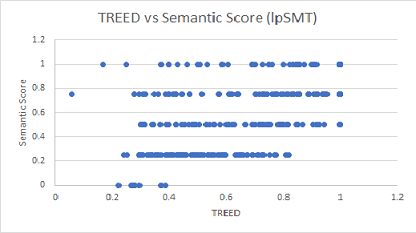
\includegraphics{img/treed_lpSMT.png}
%\label{fig:TREEDlpSMT}
%\end{figure}
%
%\begin{figure}
%\caption{TREED vs Semantic (mppSMT)}
%\centering
%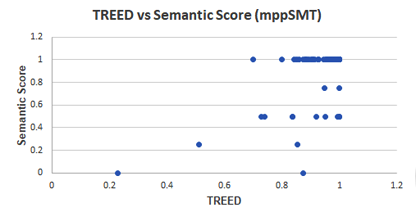
\includegraphics{img/treed_mppSMT.png}
%\label{fig:TREEDmppSMT}
%\end{figure}
%
%\subsubsection{\textbf{GVED vs Semantic}}

%There are studies that compare PDGs to measure the semantic
%similarity. PDGs capture all data and control dependence of program
%elements, and those dependencies are the keys to reflect functionality
%of source code. Therefore, GVED is expected to have the best
%correlation with Semantic score. Our results cement this argument.

%Figure \ref{fig:GVEDmppSMT} shows the scatter plots between 2 metrics:
%GVED and Semantic score when GVED is applicable. There are 240 of such
%points for the model mppSMT in the total of 375 pairs of methods, and
%75 points for lpSMT, respectively. The correlation coefficients between
%GVED and Semantic score are 0.910, 0.823, and 0.927 for the 3 models mppSMT, lpSMT, and GNMT respectively. These values show the better correlations with
%Semantic score than any of the BLEU, SED, and TREED metrics.
%
%significant improvements on both models comparing to any of the other
%3 metrics.
%
%All other three metrics have correlation coefficients with Semantic
%Score less than 0.7 while GVED achieves remarkable correlation
%coefficients of nearly 1.0 .
%
%GVED's promising result makes it an obvious choice to evaluate
%SMT-based Code Migration systems.
%

%A caveat to this is that not all migrated code is sufficiently correct
%to build the corresponding PDGs.
%
%the translated methods have too many errors that cannot be built into
%PDG, or even be compiled.
%That explains the situation in which the number of data points
%available for model lpSMT is too small to draw conclusion about the
%correlation with high confidence. Therefore, even though GVED is a
%metric with highest correlation with Semantic scores, it is not always
%applicable. To cope with its limitation while still utilizing its
%strength in correlation with semantic scores, we explore the
%combination of GVED and other metrics in our novel metric, {\model}.


%\begin{figure}
%\caption{GVED vs Semantic (lpSMT)}
%\centering
%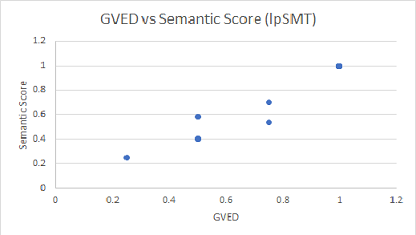
\includegraphics{img/gved_lpSMT.png}
%\label{fig:GVEDlpSMT}
%\end{figure}
%
%\begin{figure}
%\caption{GVED vs Semantic (mppSMT)}
%\centering
%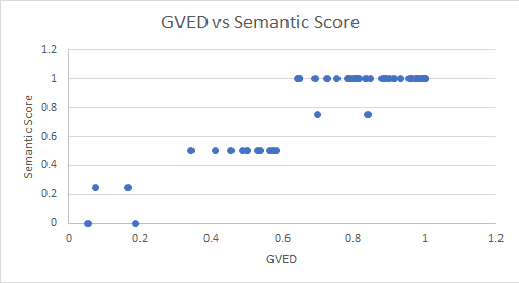
\includegraphics{img/gved_mppSMT.png}
%\label{fig:GVEDmppSMT}
%\end{figure}

